\documentclass[runningheads]{llncs}

\usepackage[T1]{fontenc}
\usepackage{graphicx}
\usepackage{hyperref}
\usepackage{color}
\usepackage{booktabs}
\usepackage{array}
\usepackage{listings}
\usepackage{float}
\usepackage[inline]{enumitem}
\usepackage{tikz}\usetikzlibrary{positioning}
\usepackage{xcolor}
\usepackage{marvosym}
\newcommand{\todo}[1]{\textcolor{red}{\textbf{[TODO: #1]}}}

\renewcommand\UrlFont{\color{blue}\rmfamily}
\usepackage{xcolor}

\begin{document}

\title{From Fragmented Records to Actionable Intelligence: LACK, a Knowledge Graph for Climate Accountability Practitioners}
\titlerunning{LACK: A Knowledge Graph for Climate Accountability}
\author{Enrico Daga\inst{1}\textsuperscript{(\Letter)} \and
Monika Mačiulienė\inst{2} \and
Gregoire Burel\inst{1} \and
Jason Carvalho\inst{1} \and\\
Arianna Graciotti\inst{3} \and
Harith Alani\inst{1} }

\authorrunning{E. Daga et al.}

\institute{Knowledge Media Institute, The Open University, Milton Keynes, UK \\
\email{\{enrico.daga, jason.carvalho, gregoire.burel, harith.alani\}@open.ac.uk} \and
Kaunas University of Technology, Kaunas, Lithuania \\ \email{monika.maciuliene@ktu.lt} \and University of Groningen, Netherlands\\ \email{a.graciotti@rug.nl}}

\maketitle
% PLACEHOLDER: Resource links block (required by submission format)
% Resource type: Knowledge Graph and Ontology
% License: CC BY 4.0
% DOI: [to be assigned]
% URL: https://climatesense-project.eu/lack/

% [INDUSTRY PAPER]
% the paper makes a claim to empower ngos cop etc... with knowledge about lobbying
% to do that, we need to look on how we put together knowledhge
% with lack we do this and that
% discussion: for industry to use it what are the pitfalls what are the opportunities and challenges
% - changes in time
% - tracing fundings
% - changes in position
% - long tail issue with entities
% - how everything is western focused

% there has been contact with influencemap on how to redistribute
% [evaluation]
% include disagreements ratio
\begin{abstract}
Climate accountability work, carried out by investigative journalists, NGOs, and watchdog organisations, depends on knowing who lobbies against climate action and how these actors are connected.
This evidence is documented in depth by platforms such as DeSmog and LobbyMap, but remains fragmented, heterogeneous, and hard to analyse at scale.
We present LACK (Lobbying Agents, Climate, and Knowledge), to our knowledge the first openly published knowledge graph of climate lobbying networks: $\sim$28k entities and $\sim$47k asserted relations ($\sim$189k after inference), built from over 2k web pages.
By making these relationships queryable, LACK is designed to support the tasks practitioners perform: tracing funding flows, tracking how actors' positions shift over time, and mapping influence networks across organisations.
We demonstrate LACK through case studies, report how domain experts assess its value, and discuss the opportunities and challenges of building such resources automatically in this domain.
\end{abstract}

%-----------------------------------------------------------------------
\section{Introduction}
\label{sec:introduction}
Lobbying networks that undermine public trust in climate science and delay effective policy action are extensively documented by investigative journalists and civil society organisations, including dedicated platforms such as DeSmog~\cite{desmog} and InfluenceMap's LobbyMap~\cite{lobbymap}, which together publish nearly 2000 profiles of people and organisations who lobby against climate action and policy.
Despite the breadth of such work, the resulting information remains siloed across heterogeneous platforms and is published primarily in long-form prose, organised around organisations' and individuals' profiles.
As a consequence, even basic questions, such as who funds a given think tank, which staff previously worked for fossil fuel companies, or which board members sit across multiple front groups, require tedious manual cross-referencing across sites with incompatible structures.
Investigative journalists, NGOs, and watchdog organisations rely on this kind of manual analysis, which does not scale.
Representing this domain as a knowledge graph makes such relational knowledge explicit and queryable at scale.

In this paper, we present LACK (Lobbying Agents, Climate, and Knowledge), a knowledge graph of persons and collectives involved in lobbying against climate science and policy, built from over 2k source documents and guided by a purpose-built lightweight ontology.
We make three contributions.
First, we present the LACK resource: a purpose-built vocabulary covering the key relation types in the climate lobbying domain, and a knowledge graph of typed relations between persons and organisations, extracted from authoritative sources, linked to Wikidata and DBpedia, and published as Linked Open Data.
Second, we demonstrate the analytical value of LACK through case studies that surface connections spanning multiple independent sources, and we assess the resource both for its coverage of the competency questions behind its design and through a survey of domain experts in investigative journalism and climate accountability.
Third, drawing on both the construction process and this expert engagement, we contribute an analysis of the opportunities and open challenges of building such resources automatically in this domain, including temporal change, funding traceability, shifting positions, long-tail entities, and geographic skew.

The remainder of this paper is structured as follows.
Section~\ref{sec:related} situates LACK in the related literature.
Section~\ref{sec:lack} describes how LACK is built and what it contains, covering the ontology, the extraction process, and the resulting resource.
Section~\ref{sec:evaluation} reports the case studies and the expert evaluation.
Section~\ref{sec:discussion} discusses the opportunities and open challenges of building and using such a resource in practice, and concludes with directions for future work.
\section{Background and Related Work}
\label{sec:related}

Corporate lobbying has demonstrable consequences for climate policy outcomes.
Brulle~\cite{brulle2018climate} maps US climate-lobbying expenditure across industry sectors, and Meng and Rode~\cite{meng2019social} estimate that lobbying lowered the probability of enacting the Waxman--Markey Cap-and-Trade Bill (a crucial US climate action bill) by 13 percentage points, with an estimated welfare loss of roughly \$60 billion.
More recently, Leippold, Sautner and Yu~\cite{leippold2024corporate} document a \emph{camouflaging trend}, whereby firms increasingly conceal climate lobbying behind opaque legislative references, while Baehr, Bare and Heddesheimer~\cite{baehr2026climate} show across more than 11{,}000 firms that earnings-call \emph{climate exposure} systematically predicts whether, how much, and where a firm lobbies.
Understanding lobbying therefore requires more than aggregate spending figures: it requires modelling the underlying network of actors, funders, and affiliations through which climate-policy influence is organised and exerted.

\begin{sloppypar}
The resources practitioners rely on today partly address the documentation challenge but stop short of making this network queryable.
DeSmog~\cite{desmog} profiles individuals and organisations involved in denial and lobbying; LobbyMap~\cite{lobbymap} tracks corporate engagement with climate policy; Skeptical Science~\cite{skepticalscience} curates statements attributed to prominent misinformation actors; and Oreskes and Conway~\cite{oreskes2011merchants} analyse the strategies used to manufacture doubt about scientific consensus.
These resources are invaluable but heterogeneous, siloed, and not interlinked in any form amenable to computational analysis, leaving cross-source questions to manual effort.
Concurrent efforts such as the UCL \emph{AI-Powered Climate Lobbying Database}~\cite{uclclimatelobbying} reflect the recognised need for better support, automating text extraction and network analysis with large language models.
\end{sloppypar}

In the Semantic Web community, CimpleKG~\cite{burel2024cimplekg} provides a continuously updated knowledge graph on misinformation and fact-checks across domains, currently being extended within the ClimateSense project~\cite{climatesense} with climate-specific classifiers, while ClimaFactsKG~\cite{burel2025climafactskg} structures scientific evidence countering climate misinformation; both, however, target claim verification rather than lobbying actor networks.
Knowledge graphs have also been adopted as infrastructure for investigative journalism~\cite{opdahl2022semantic,gallofre2022jkp,berven2020kg,alexander2023manifesto,motta2025epistemology} and for political discourse, including European Parliament debates~\cite{van2016debates} and the digitised Canadian parliamentary record~\cite{beelen2017digitization}, but these model news content, events, or formal proceedings rather than the off-stage networks of funding, affiliation, and personnel through which lobbying influence operates.
Constructing such a graph relies on well-studied entity resolution and linking techniques~\cite{christophides2020er,sevgili2022neural,ayoola2022refined}, increasingly addressed with large language models that match or exceed supervised baselines without task-specific training~\cite{peeters2025llmem}; this fits the climate-lobbying setting, where many mentions are long-tail entities absent from general-purpose knowledge bases.
What is still missing is a machine-readable representation of the actors and relationships at the core of climate lobbying, and LACK fills this gap as a Wikidata-linked knowledge graph built from investigative sources and published as Linked Open Data.
<<<<<<< HEAD
\begin{figure}[t]
    \centering
    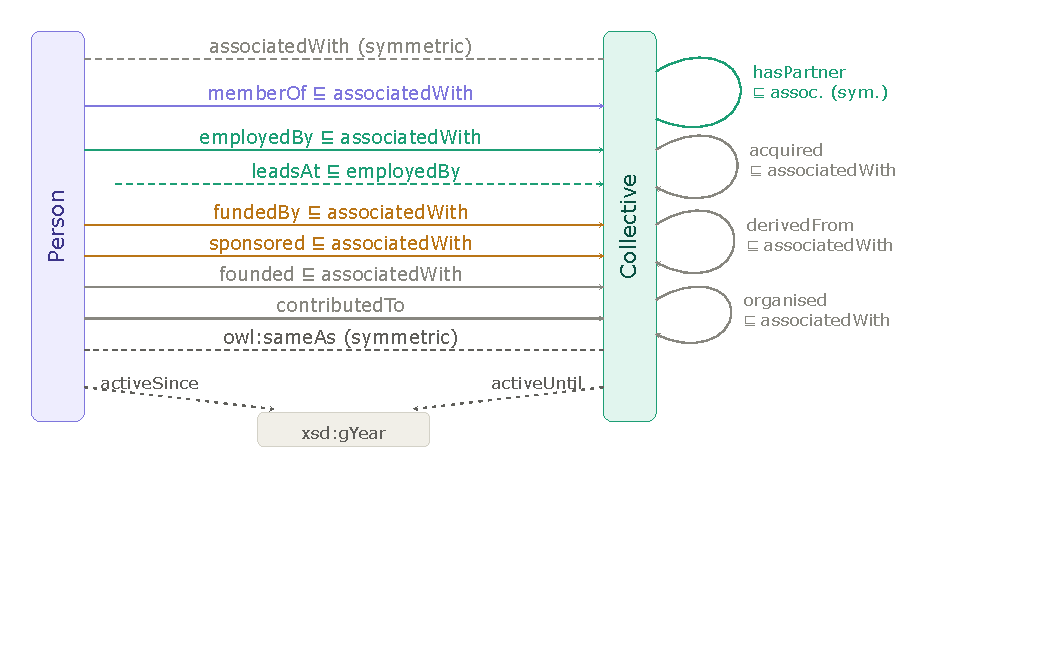
\includegraphics[trim={0 3.5cm 2cm 0cm},clip,width=\textwidth]{figures/lack-ontology-diagram.pdf}
    \vspace{-0.3cm}\caption{Schema diagram of the LACK ontology.}
\label{fig:ontology}\vspace{-0.3cm}
\end{figure}

\section{The LACK Resource}
=======

\begin{figure}[t]
    \centering
    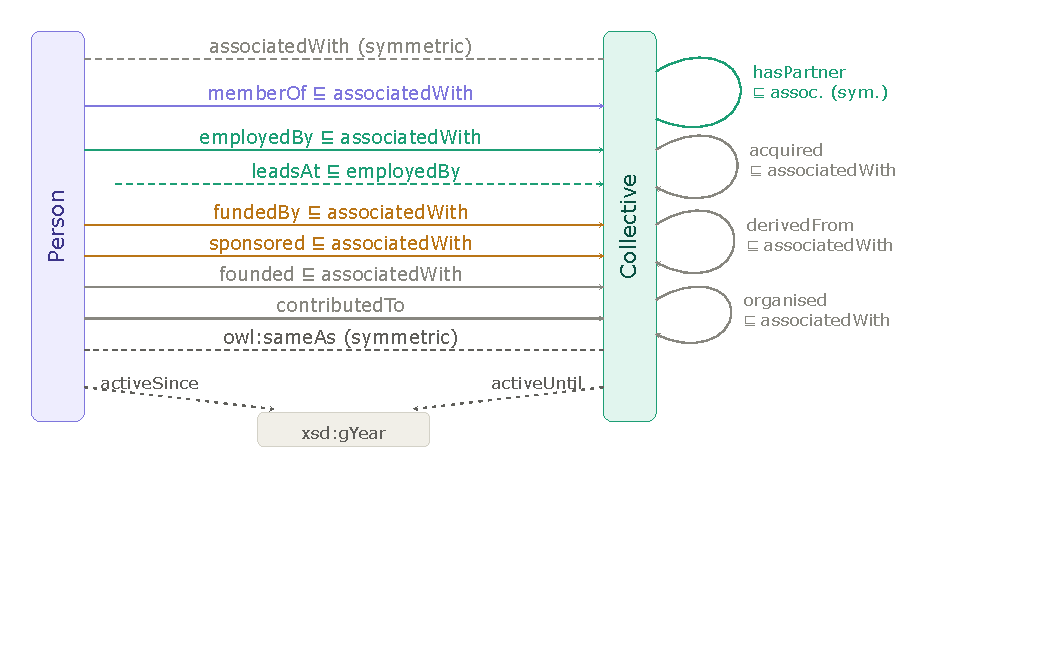
\includegraphics[trim={0 3.5cm 2cm 0.5cm},clip,width=\textwidth]{figures/lack-ontology-diagram.pdf}
    \vspace{-0.5cm}\caption{Schema diagram of the LACK ontology.}
\label{fig:ontology}\vspace{-0.5cm}
\end{figure}
\section{The LACK Knowledge Graph}
>>>>>>> 2cd6a84036c92e32b01883403f8af4ab7aa95d27
\label{sec:lack}

\vspace{-0.3cm}\paragraph{Sources.}
LACK was built from the two most comprehensive English-language databases dedicated to climate-lobbying actors\footnote{Pages accessed in December 2025.}.
The \textbf{DeSmog Climate Disinformation Database}~\cite{desmog}, maintained by DeSmog (an international investigative journalism organisation founded in 2006 and philanthropically funded), profiles individuals and organisations involved in climate denial, typically covering positions on climate science, affiliations, funding sources, and public statements; we collected all 943 profile pages.
\textbf{LobbyMap}~\cite{lobbymap}, maintained by InfluenceMap (an independent non-profit think tank founded in 2015), provides analyst-scored, IPCC-benchmarked assessments of corporate and industry-association engagement with climate policy for approximately 1{,}000 companies and 330 associations; we collected the 964 LobbyMap Scores profiles plus 338 further organisations referenced within them (1,302 pages total).
The two sources are complementary: DeSmog focuses on individuals and think tanks involved in disinformation, while LobbyMap covers groups engaging with policy; well-known actors appear in both.
The pages were collected using SPARQL Anything~\cite{daga2021opinionated}, querying DeSmog's HTML pages' index and the LobbyMap leaderboard JSON feed.

\begin{sloppypar}
\vspace{-0.3cm}\paragraph{Ontology.}
The LACK ontology (Figure~\ref{fig:ontology}) was designed bottom-up from the investigative sources: recurring information types were formalised as twelve competency questions (CQ1--CQ12), which drove the design of both the schema and the extraction process\footnote{\url{https://climatesense-project.eu/lack/ontology.html}}.
<<<<<<< HEAD
A guiding principle was to represent only what could be reliably and automatically extracted, deliberately excluding relation types (such as fine-grained roles) that could not be produced with sufficient confidence; this also motivated a purpose-built vocabulary, since general-purpose vocabularies such as Schema.org\footnote{\url{http://schema.org}} lack equivalents for lobbying-specific relations and would fragment the graph through intermediary role nodes.
The ontology defines two top-level classes, \texttt{lack:Person} (an individual) and \texttt{lack:Collective} (any group organised around a shared purpose, deliberately broad to accommodate events, journals, campaigns, and networks alongside organisations).
=======
The LACK ontology (Figure~\ref{fig:ontology}) was designed following the NeOn methodology~\cite{suarez2011neon}, with one deliberate adaptation: rather than eliciting requirements from domain experts directly, we treated the investigative sources themselves as a proxy for user needs, assuming that platforms such as DeSmog and LobbyMap already encode the questions their users care about.
To guide design, we derived twelve \textit{competency questions} (following~\cite{suarez2011neon}) from information content of the source pages, and re-engineered those sources, as non-ontological resources, into a domain schema\footnote{\url{https://climatesense-project.eu/lack/ontology.html}}; we revisit and confirm this assumption through the expert evaluation in Section~\ref{sec:evaluation}.
Practitioner requirements were not elicited at design time, so the schema is bounded by what the sources themselves document; the expert survey (Section~\ref{sec:eval:experts}) provides post-hoc validation and, as we discuss there, marks that boundary.
% The LACK ontology (Figure~\ref{fig:ontology}) was designed following the NeOn methodology~\cite{suarez2011neon}, combining a requirements specification expressed as twelve competency questions (CQ1--CQ12) with the re-engineering of our investigative sources, treated as non-ontological resources, into a domain schema\footnote{\url{https://climatesense-project.eu/lack/ontology.html}}.
% A guiding principle was to represent only what could be reliably and automatically extracted, 
Crucially, relation types that could not be derived from the sources are excluded.
We evaluated general-purpose vocabularies such as Schema.org~\cite{schemaorg} or the W3C Organisation ontology, which don't have lobbying-specific relations and/or would fragment the graph through intermediary role nodes.
The ontology defines two top-level classes, \texttt{lack:Person} (an individual) and \texttt{lack:Collective} (any group organised around a shared purpose, deliberately broad to accommodate events, journals, campaigns, and groups alongside organisations)\footnote{We note that alignments with \texttt{foaf:Agent} and \texttt{foaf:Person} are possible for \texttt{lack:Person} but not for \texttt{lack:Collective}.}.
>>>>>>> 2cd6a84036c92e32b01883403f8af4ab7aa95d27
Each relation is defined with a domain, range, and inverse, organised in a hierarchy rooted at the symmetric catch-all \texttt{lack:associatedWith}.
Relationships can be time-bounded, captured through entity-level bounds (\texttt{lack:activeSince}/\texttt{lack:activeUntil}) and relation-level annotations via reification~\cite{rdfprimer}, where each temporally annotated triple is reified as an \texttt{rdf:Statement} carrying \texttt{lack:since}/\texttt{lack:until}; reification was chosen over RDF-star for broad compatibility with current RDF tooling.
Provenance and source attribution reuse PROV-O~\cite{provo} and Dublin Core Terms~\cite{dcterms}, linking each statement to the extraction activity and to the source web page.\end{sloppypar}

<<<<<<< HEAD
\paragraph{Construction.}
The knowledge graph is produced from the raw extraction outputs by a pipeline implemented with SPARQL Anything~\cite{asprino2023knowledge}, reproducible from the source CSVs~\cite{lack-kgc}.
Relations are first extracted from the source pages by prompting Gemini 2.5 Flash~\cite{gemini25} with the allowed relation types and a strict JSON schema, then linked to authoritative identifiers through a hybrid entity-linking step combining Wikidata candidate retrieval, LLM-based disambiguation, and a web-search fallback, with Llama 3.3 70B~\cite{llama33} used at scale~\cite{lack-re,lack-el}.
Construction then proceeds in five phases: (i) the 152 distinct surface-form relation types (90,145 instances) are aligned to ontology properties; (ii) stable IRIs are minted per entity by hashing the highest-priority identifier available (Wikidata QID, then Wikipedia, then web page, then surface form with source URL), each typed as \texttt{lack:Person} or \texttt{lack:Collective} with a granular subtype and, where available, \texttt{owl:sameAs} links to Wikidata and DBpedia; (iii) each relation is written as a typed triple plus a reified statement carrying evidence and temporal bounds; (iv) PROV-O provenance is attached; and (v) ontology entailments (inverse pairs, sub-property promotions, symmetric closure) are materialised, growing the graph from 47,450 asserted relations to 188,862 triples.
=======
\vspace{-0.3cm}\paragraph{Construction.}
Relations are first extracted from the source pages by prompting Gemini 2.5 Flash~\cite{gemini25} with the allowed relation types and a strict JSON schema, then linked to authoritative identifiers through a hybrid entity-linking step combining Wikidata candidate retrieval, LLM-based disambiguation, and a web-search fallback, with Llama 3.3 70B~\cite{llama33} used at scale (see supplementary material~\cite{lack-re,lack-el}).
Construction encompasses five phases: (i) the 152 distinct surface-form relation types (90,145 instances) are aligned to ontology properties; (ii) stable IRIs are minted per entity by hashing the highest-priority identifier available (Wikidata QID, then Wikipedia, then web page, then surface form with source URL), each typed as \texttt{lack:Person} or \texttt{lack:Collective} with a granular subtype and, where available, \texttt{owl:sameAs} links to Wikidata and DBpedia; (iii) each relation is written as a typed triple plus a reified statement carrying evidence and temporal bounds; (iv) PROV-O provenance is attached; and (v) ontology entailments (inverse pairs, sub-property promotions, symmetric closure) are materialised, growing the graph from 47,450 \emph{asserted} relation triples, each evidenced by a source page, to 188,862 relation triples in total; the additional triples are entailed rather than independently extracted, and we keep the two counts separate throughout.
The knowledge graph is produced from the raw extraction outputs by a pipeline implemented with SPARQL Anything~\cite{sparqlanything} (reproducible at~\cite{lack-kgc}).
>>>>>>> 2cd6a84036c92e32b01883403f8af4ab7aa95d27

\vspace{-0.3cm}\paragraph{Availability and Maintenance.}
The LACK ontology and knowledge graph are published as Linked Open Data under a Creative Commons Attribution Non-Commercial 4.0 International (CC BY NC 4.0) licence.
Version 1.1 was released in April 2026 and is accessible at \url{https://climatesense-project.eu/lack/} as a Turtle dump (\texttt{KG.ttl}), a live SPARQL endpoint powered by QLever\footnote{\url{https://sparql.climatesense.kmi.tools/climatesense}}, and an interactive exploration interface.
Table~\ref{tab:kg-stats} summarises statistics; a full breakdown is on the LACK website.
The ontology is separately available under the persistent namespace \url{https://purl.net/climatesense/lack/ns#}, and the dataset is archived on Zenodo~\cite{lack}.
The resource is maintained by KMi and guaranteed available for at least five years under funder open data policy. 
Infrastructure for continuos updates is currently under development.
% \paragraph{Disclaimer.}
% LACK reorganises information from third-party investigative sources; the authors do not endorse or assume responsibility for the original claims, and the relations published surface structural connections rather than allegations against any named party.

\begin{table}[t]
\centering
\caption{LACK KG statistics. Inferred triples overlap with asserted ones, so the post-inference count is not their sum. The graph total additionally includes reified statements, provenance, and \texttt{owl:sameAs}/\texttt{rdfs:seeAlso} links.}
% \caption{Statistics. Inferred relation triples overlap with asserted ones (e.g.\ \texttt{associatedWith} may also be asserted), so the post-inference relation count is not their sum. Totals includes reified statements, provenance, and \texttt{owl:sameAs}/\texttt{rdfs:seeAlso}.}
\label{tab:kg-stats}
\small
\begin{tabular}{lr}
\toprule
\textbf{Dimension} & \textbf{Count} \\
\midrule
Entities (Person / Collective / Total)
  & 10,370 / 17,604 / \textbf{27,945} \\
\quad Wikidata links (Person / Collective / Total)
  & 2,911 / 5,369 / \textbf{8,280} \\
\quad DBpedia links (Person / Collective / Total)
  & 3,516 / 5,210 / \textbf{8,726} \\
\midrule
Relations triples, asserted          & 47,450 \\
Relations triples, after inference   & \textbf{188,862} \\
All triples in the graph     & \textbf{213,147} \\
Evidence (Desmog / LobbyMap / InfluenceMap / Total)
  & 943 / 964 / 338 / \textbf{2,245} \\
\bottomrule
\end{tabular}
\vspace{-0.5cm}
\end{table}

% \begin{table}[t]
% \centering
% \caption{LACK KG statistics.}
% \label{tab:kg-stats}
% \small
% \begin{tabular}{lr}
% \toprule
% \textbf{Dimension} & \textbf{Count} \\
% \midrule
% Entities (Person / Collective / Total)
%   & 10,370 / 17,604 / \textbf{27,945} \\
% \quad Wikidata links (Person / Collective / Total)
%   & 2,911 / 5,369 / \textbf{8,280} \\
% \quad DBpedia links (Person / Collective / Total)
%   & 3,516 / 5,210 / \textbf{8,726} \\
% \midrule
% Relations (Asserted / Inferred / Total)
%   & 47,450 / 142,737 / \textbf{213,147} \\
% Evidence (Desmog / LobbyMap / InfluenceMap / Total)
%   & 943 / 964 / 338 / \textbf{2,245} \\
% \bottomrule
% \end{tabular}
<<<<<<< HEAD
% \end{table}
=======
% \end{table}
>>>>>>> 2cd6a84036c92e32b01883403f8af4ab7aa95d27

\section{Demonstration and Evaluation}
\label{sec:evaluation}
A resource intended for accountability work must be trustworthy before it can be useful.
We therefore assess LACK in four steps: the accuracy of its extracted relations and entity links (Section~\ref{sec:eval:quality}), its coverage of the competency questions that drove its design (Section~\ref{sec:eval:coverage}), the analyses it enables through case studies (Section~\ref{sec:eval:cases}), and its perceived value to domain experts (Section~\ref{sec:eval:experts}).

\subsection{Extraction and Linking Quality}
\label{sec:eval:quality}
We evaluated relation extraction on a sample of 300 relations drawn from 8 randomly selected DeSmog profile pages.
Three annotators (the authors) worked in pairs, each covering approximately 100 relations, with disagreements resolved by discussion, assessing each relation for truthfulness (is it supported by the source page?), validity (is the relation type and its domain and range correctly applied?), and temporal correctness\footnote{Full annotation guidelines: \url{https://bit.ly/lack_42bhqzl}.}.
Truthfulness accuracy is 0.93 (0.99 with partial credit), validity 0.91 (0.95 with partial), and temporal correctness 0.80 (0.91 with partial), where partial credit captures approximately correct extractions.
Partly correct answers mostly stem from sub-role conflation (e.g.\ \texttt{is president of} used for a vice-president) and from organisation-level relations misapplied to person-organisation pairs; temporal correctness is the weakest dimension, with errors from missing dates and ambiguity between point-in-time and interval information.

Entity linking was evaluated on 225 entities from the same pages, against a curated gold standard\footnote{Gold standard preparation: \url{https://bit.ly/lack_3QQPRsD}.} produced by four annotators with disagreements resolved by discussion.
Accuracy is high across the primary output fields (Wikidata URI and Wikipedia URL both 0.88, entity subtype 0.86, parent entity 0.94), with balanced precision and recall for the two precisely-definable fields (0.93/0.85 and 0.88/0.88); the weakest field is the canonical web page (0.49 precision), reflecting the difficulty of identifying a single web presence for an entity.
Of the 27,945 entities, 36.5\% are linked to Wikidata or DBpedia and 63.5\% remain without an external identifier.
This high NIL rate is a domain characteristic rather than a pipeline failure: the climate-lobbying ecosystem is densely populated with minor think-tank staff, obscure consultants, short-lived coalitions, and regional trade bodies absent from general-purpose knowledge bases.
By contrast, entities documented by both sources, those prominent enough to appear independently in DeSmog and LobbyMap, are linked at 95.7\% (488 of 510), confirming that the pipeline reliably grounds well-known actors.

\subsection{Coverage of Competency Questions}
\label{sec:eval:coverage}
We assess the extent to which the graph answers the competency questions that drove its design.
For each CQ, Table~\ref{tab:coverage} reports the ontology relation(s) involved, triple counts before and after inferencing, the distinct entities affected, and the resulting coverage ratio (entities affected over 27,974 total; for the temporal CQ10, reified statements carrying \texttt{lack:since}/\texttt{lack:until} over 51,848 total).
We classify CQs into three tiers using natural breaks in the distribution of coverage ratios: the largest gap (7.5\,pp, between 12.2\% and 4.7\%) separates \textbf{Weak} from the rest, and the next (7.2\,pp, between 22.8\% and 15.6\%) separates \textbf{Strong} from \textbf{Moderate}.
CQ9 is reported separately, since \texttt{associatedWith} is the top-level relation and its coverage is inflated by inference; CQ1 is degenerate (every entity satisfies it) and reported as N/A.
Coverage is solid across the core transparency and network-structure questions, with employment, membership, leadership, and statement-level temporal annotation all in the Strong tier.
The most striking result is network reach (CQ9): after inferencing, 93.5\% of entities are reachable via \texttt{associatedWith}, turning a sparse set of assertions into a near-complete connectivity structure.
Temporal coverage is partial: statement-level annotation (CQ10) reaches the Strong tier, while entity-level bounds (CQ11) cover only 2.6\% of entities and should be treated as supplementary.
Founding relations (CQ7) remain sparse, reflecting the difficulty of reliably extracting founding events.

\begin{table}[t]
\centering
\caption{Mapping of competency questions to ontology relations, triple counts (before and after inferencing), affected entities, coverage ratio, and tier.}
\label{tab:coverage}
\begin{tabular}{p{0.07\textwidth} >{\raggedright}p{0.18\textwidth} >{\raggedright}p{0.18\textwidth} >{\raggedright}p{0.22\textwidth} >{\raggedright}p{0.11\textwidth} >{\raggedright}p{0.08\textwidth} p{0.10\textwidth}}
\hline
\textbf{CQ} & \textbf{RQ (summary)} & \textbf{Relation(s)} & \textbf{Triples (before$\to$after)} & \textbf{Entities} & \textbf{(\%)} & \textbf{Tier} \\
\hline
CQ1  & Who is involved?           & (entities)                                      & 27,974 $\to$ 27,974   & 27,974 & 100.0 & N/A \\
CQ2  & How are actors funded?     & \texttt{fundedBy} / \texttt{hasFunder}        & 5,210 $\to$ 10,420    & 3,421  & 12.2  & Moderate \\
CQ3  & Who are the members?       & \texttt{memberOf} / \texttt{hasMember}        & 13,469 $\to$ 26,912   & 9,718  & 34.7  & Strong \\
CQ4  & Who leads organisations?   & \texttt{leadsAt} / \texttt{hasLeader}         & 5,639 $\to$ 11,278    & 6,383  & 22.8  & Strong \\
CQ5  & Employment history?        & \texttt{employedBy} / \texttt{hasEmployee}    & 5,463 $\to$ 21,276    & 10,943 & 39.1  & Strong \\
CQ6  & Structural connections?    & \texttt{hasPartner}, \texttt{sponsored}       & 5,686 $\to$ 8,013     & 4,365  & 15.6  & Moderate \\
CQ7  & Who founded a group?       & \texttt{founded} / \texttt{wasFoundedBy}      & 73 $\to$ 146          & 108    & 0.4   & Weak \\
CQ8  & Derivative organisations?  & \texttt{derivedFrom} / \texttt{hasDerivation} & 1,922 $\to$ 2,883     & 1,310  & 4.7   & Weak \\
CQ9  & Network reach?             & \texttt{associatedWith}                       & 3,216 $\to$ 91,219    & 26,169 & 93.5  & (Strong) \\
CQ10 & Networks change over time? & \texttt{since} / \texttt{until} (reif.)       & 14,361 $\to$ 14,361   & ---    & 27.7  & Strong \\
CQ11 & When were actors active?   & \texttt{activeSince} / \texttt{activeUntil}   & 836 $\to$ 836         & 734    & 2.6   & Weak \\
\hline
\end{tabular}
\vspace{-0.5cm}
\end{table}

\subsection{Case Studies}
\label{sec:eval:cases}
\begin{sloppypar}
\paragraph{Integrating independent sources.}
LACK's central value is making visible connections that no single source exposes.
Each of the following examples joins two statements, drawn from different sources, that share a bridge entity; the connections are structural, derived from public data, and presented as research leads rather than allegations\footnote{The connections are structural and do not imply wrongdoing, shared intent, or direct collaboration.}.
In the first, InfluenceMap records Darren Woods leading Exxon (\texttt{lack:leadsAt}) while DeSmog records Exxon sponsoring the Heartland Institute (\texttt{lack:sponsored}), a think tank associated with climate science denial; joining the two relations in a single SPARQL query links a named corporate officer to a denial organisation through his employer.
In the second, DeSmog records a partnership between Cambridge Analytica and BP (\texttt{lack:hasPartner}) while InfluenceMap records BP's membership of the Business Council of Australia (\texttt{lack:memberOf}); the two facts originate in different investigative contexts and share only BP, yet LACK surfaces a cross-domain, cross-jurisdictional connection invisible to either source alone.
\end{sloppypar}

\begin{sloppypar}
\paragraph{Cross-referencing with COP30.}
Pairing LACK with an external source of named climate-policy agents enables a further family of analyses.
We cross-referenced LACK's 1,000 most heavily-described \texttt{lack:Collective} entities with the COP30 participant list via heuristic label matching.
Of 944 distinct delegate matches, roughly 70\% flow through observer accreditation channels, 18\% appear in high-income national delegations, and only 43 in lower- or low-income country delegations.
Within the most densely connected entities, the US climate countermovement (Heartland, Cato, ALEC, Heritage, Manhattan Institute) is almost entirely absent from COP30, with only three (US Chamber of Commerce, Shell, ExxonMobil) present at all.
The cross-reference surfaces two findings invisible to either resource alone: the US climate countermovement does not engage with the UNFCCC track, and observer accreditation, rather than national delegation, is the dominant channel through which LACK-tracked organisations participate in COP.
\end{sloppypar}

\subsection{Expert Evaluation}
\label{sec:eval:experts}
A 14-question online questionnaire was distributed via purposive sampling to researchers, fact-checkers, investigative journalists, NGO professionals, and policy analysts working on climate lobbying networks, across 25 organisational groups spanning academic networks, fact-checking organisations, investigative outlets, NGOs, and international bodies.
Of 68 invitations, 9 were completed (13.2\%); while small, the sample spans the primary user communities, and the consistency of responses across professional backgrounds lends confidence to the findings.
Respondents unanimously rated both the overall value of such a resource and the ability to search across multiple sources at M=4.62 on a 5-point scale, directly validating LACK's integration approach.

On priority relation types, funding flows received the highest mean rating (M=4.75), followed by employment (M=4.50), and membership, sponsorship, and founding (each M=4.38).
Cross-referencing with Table~\ref{tab:coverage}, employment (CQ5) and membership (CQ3) fall in the Strong tier, well-matched to expert demand; funding (CQ2), the top-rated category, is only Moderate (12.2\%), consistent with respondents' own remarks on how hard funding information is to obtain.
Leadership (CQ4, M=4.25) is similarly well served (Strong, 22.8\%), while founding relations (CQ7) are the most significant mismatch (Weak), identifying founding data as a priority for enrichment.
Temporal information was rated M=3.88 and flagged by half the respondents as one of the hardest dimensions to find, consistent with the partial temporal coverage reported above.
Several respondents identified gaps outside LACK's current scope, notably direct connections to the political sphere and a need to distinguish intermediary actor types (lobby consultancies, law firms, PR agencies), and recommended integrating further sources such as the EU Transparency Register, LobbyFacts, SourceWatch, and OpenSecrets.
We return to these gaps, and to the broader challenges they raise, in Section~\ref{sec:discussion}.
\vspace{-0.3cm}\section{Discussion and Outlook}\vspace{-0.3cm}
\label{sec:discussion}\begin{sloppypar}
Building LACK showed that valuable info can be automatically extracted, integrated and enriched with semantics.
Connections that are invisible within any single source become queryable once the sources are represented in a common graph, and this cross-source bridging is precisely what practitioners told us they value most.
We see no reason this approach should remain specific to climate lobbying.
The same approach, harvesting heterogeneous investigative documentation, extracting typed relations with large language models, and grounding entities against open knowledge bases, could in principle support accountability work in other domains, such as public-health lobbying or defence procurement.
Demonstrating this generalisation is an aim of our ongoing work.\end{sloppypar}

At the same time, the construction process surfaces challenges that are characteristic of this domain.
Lobbying networks are dynamic: positions, affiliations, and roles change over time, yet temporal information is the dimension our evaluation and our experts both found hardest to capture, and entity-level activity bounds remain sparse.
Funding is the relation practitioners most want and one of the hardest to extract reliably, since funding ties are often disclosed obliquely or not at all, as our experts also noted.
The long tail of minor actors, obscure consultants, short-lived coalitions, regional trade bodies, drives the high proportion of entities without external identifiers; rather than a mere limitation, this is an open research problem, since enriching and disambiguating long-tail entities absent from general-purpose knowledge bases is an active challenge for automatic knowledge graph construction~\cite{graciotti2025lost}.
The reliance on English-language sources introduces a geographic and linguistic skew, visible in our COP30 cross-reference, where actors from lower-income countries are markedly under-represented.

Turning a resource into something practitioners can adopt raises questions beyond extraction quality.
LACK reorganises information produced by investigative organisations who invest considerable effort in it, and respecting that effort is of primary importance: we followed DeSmog's republishing guidelines and complied with the redistribution terms we obtained from InfluenceMap, and we publish LACK under a Creative Commons Attribution-NonCommercial licence.
In an era when large commercial actors routinely ingest others' content without credit, a BY-NC licence preserves attribution and reserves commercial rights to the original data owners, which we hope makes it easier, not harder, for further investigative organisations to contribute to a shared LACK data space.
The gaps our experts identified, direct links to the political sphere, finer distinctions between intermediary actor types such as consultancies and PR agencies, and integration of further sources such as the EU Transparency Register and OpenSecrets, define our agenda for that growth.

In summary, we have presented LACK, to our knowledge the first openly published knowledge graph that turns fragmented investigative records on climate lobbying into a queryable resource, demonstrated its analytical value, and assessed both its quality and its reception among the practitioners it is meant to serve.
By releasing LACK as an open, attribution-preserving resource, we hope to invite the organisations whose work it builds on to help extend it, growing it from a knowledge graph into a shared data space for climate accountability.
\vspace{-0.5cm}
%-----------------------------------------------------------------------

\bibliographystyle{splncs04}
\bibliography{main}

\end{document}
